\documentclass{standalone}
\usepackage{tikz}
\usetikzlibrary{patterns, positioning}


\begin{document}
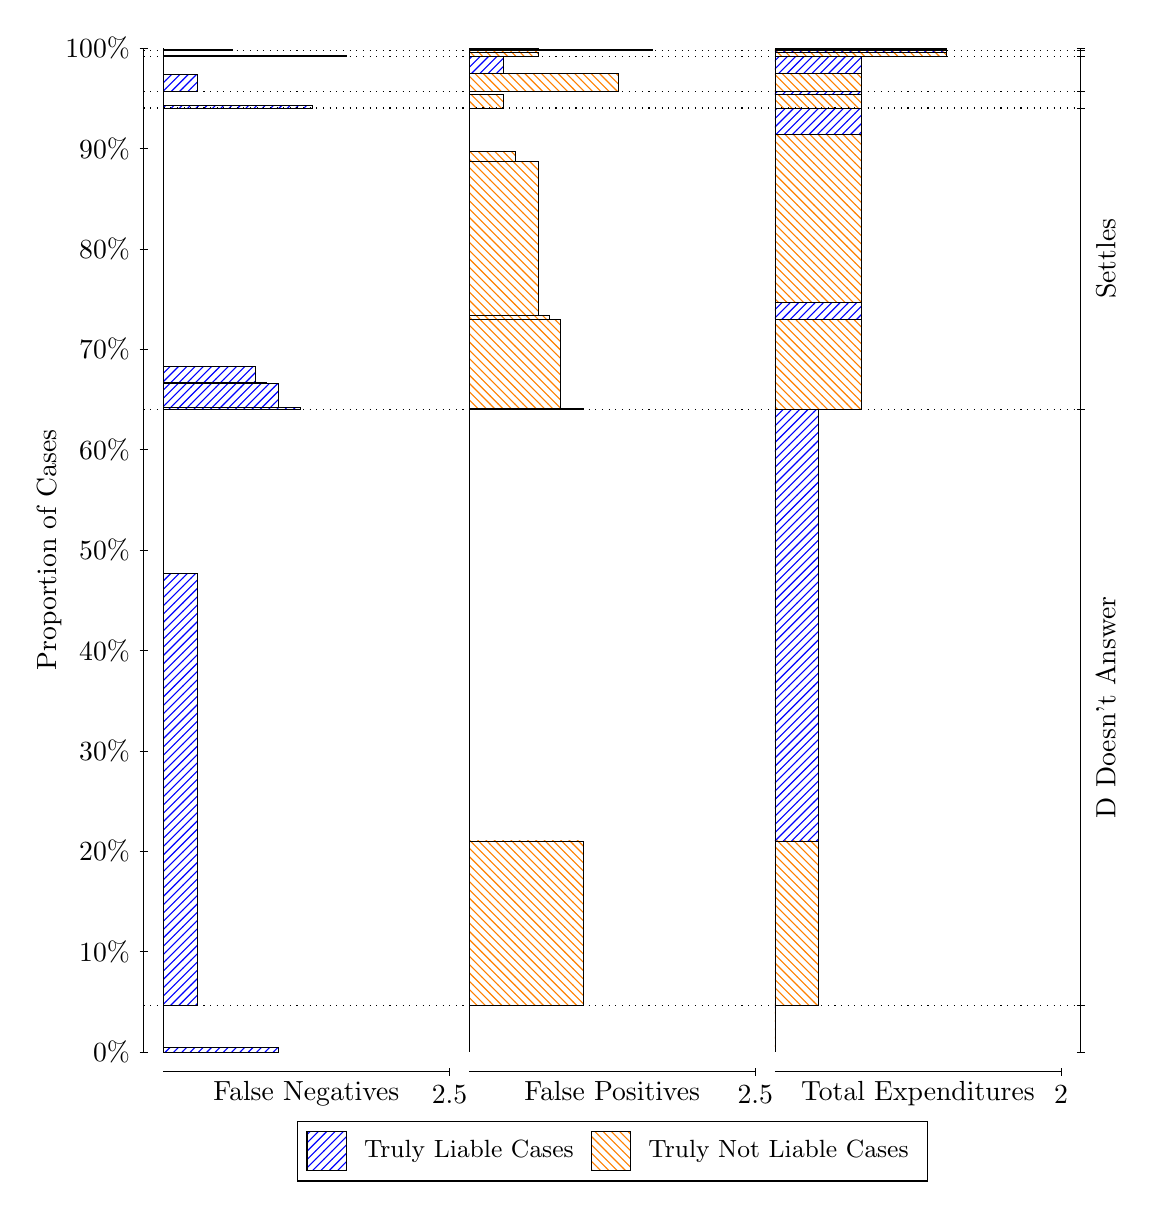
\begin{tikzpicture}
\draw[black, very thin] (1.5,1.75) -- (1.5,14.5);
\node[rotate=90, text=black, anchor=center] at (0.3, 8.125) {Proportion of Cases};
\draw[black, very thin] (1.45,1.75) -- (1.55,1.75);
\node[text=black, anchor=east] at (1.45, 1.75) {0\%};
\draw[black, very thin] (1.45,3.025) -- (1.55,3.025);
\node[text=black, anchor=east] at (1.45, 3.025) {10\%};
\draw[black, very thin] (1.45,4.3) -- (1.55,4.3);
\node[text=black, anchor=east] at (1.45, 4.3) {20\%};
\draw[black, very thin] (1.45,5.575) -- (1.55,5.575);
\node[text=black, anchor=east] at (1.45, 5.575) {30\%};
\draw[black, very thin] (1.45,6.85) -- (1.55,6.85);
\node[text=black, anchor=east] at (1.45, 6.85) {40\%};
\draw[black, very thin] (1.45,8.125) -- (1.55,8.125);
\node[text=black, anchor=east] at (1.45, 8.125) {50\%};
\draw[black, very thin] (1.45,9.4) -- (1.55,9.4);
\node[text=black, anchor=east] at (1.45, 9.4) {60\%};
\draw[black, very thin] (1.45,10.675) -- (1.55,10.675);
\node[text=black, anchor=east] at (1.45, 10.675) {70\%};
\draw[black, very thin] (1.45,11.95) -- (1.55,11.95);
\node[text=black, anchor=east] at (1.45, 11.95) {80\%};
\draw[black, very thin] (1.45,13.225) -- (1.55,13.225);
\node[text=black, anchor=east] at (1.45, 13.225) {90\%};
\draw[black, very thin] (1.45,14.5) -- (1.55,14.5);
\node[text=black, anchor=east] at (1.45, 14.5) {100\%};

\draw[black, very thin] (13.4,1.75) -- (13.4,14.5);
\draw[black, very thin] (13.35,1.75) -- (13.45,1.75);
\node[anchor=west] at (13.35, 1.75) {};
\draw[black, very thin] (13.35,2.3431) -- (13.45,2.3431);
\node[anchor=west] at (13.35, 2.3431) {};
\draw[black, very thin] (13.35,9.9124) -- (13.45,9.9124);
\node[anchor=west] at (13.35, 9.9124) {};
\draw[black, very thin] (13.35,13.738) -- (13.45,13.738);
\node[anchor=west] at (13.35, 13.738) {};
\draw[black, very thin] (13.35,13.945) -- (13.45,13.945);
\node[anchor=west] at (13.35, 13.945) {};
\draw[black, very thin] (13.35,14.394) -- (13.45,14.394);
\node[anchor=west] at (13.35, 14.394) {};
\draw[black, very thin] (13.35,14.467) -- (13.45,14.467);
\node[anchor=west] at (13.35, 14.467) {};
\draw[black, very thin] (13.35,14.5) -- (13.45,14.5);
\node[anchor=west] at (13.35, 14.5) {};

\draw[black, very thin, pattern color=blue, pattern=north east lines] (1.75,1.75) rectangle (3.2033,1.8124);
\draw[black, very thin, pattern color=orange, pattern=north west lines] (1.75,1.8124) rectangle (1.75,2.3431);
\draw[black, very thin, pattern color=blue, pattern=north east lines] (1.75,2.3431) rectangle (2.186,7.8235);
\draw[black, very thin, pattern color=orange, pattern=north west lines] (1.75,7.8235) rectangle (1.75,9.9124);
\draw[black, very thin, pattern color=blue, pattern=north east lines] (1.75,9.9124) rectangle (3.494,9.9333);
\draw[black, very thin, pattern color=blue, pattern=north east lines] (1.75,9.9333) rectangle (3.2033,10.238);
\draw[black, very thin, pattern color=blue, pattern=north east lines] (1.75,10.238) rectangle (3.058,10.252);
\draw[black, very thin, pattern color=blue, pattern=north east lines] (1.75,10.252) rectangle (2.9127,10.452);
\draw[black, very thin, pattern color=blue, pattern=north east lines] (1.75,10.452) rectangle (2.622,10.46);
\draw[black, very thin, pattern color=orange, pattern=north west lines] (1.75,10.46) rectangle (1.75,13.738);
\draw[black, very thin, pattern color=blue, pattern=north east lines] (1.75,13.738) rectangle (3.6393,13.768);
\draw[black, very thin, pattern color=orange, pattern=north west lines] (1.75,13.768) rectangle (1.75,13.945);
\draw[black, very thin, pattern color=blue, pattern=north east lines] (1.75,13.945) rectangle (2.186,14.166);
\draw[black, very thin, pattern color=orange, pattern=north west lines] (1.75,14.166) rectangle (1.75,14.394);
\draw[black, very thin, pattern color=blue, pattern=north east lines] (1.75,14.394) rectangle (4.0753,14.411);
\draw[black, very thin, pattern color=orange, pattern=north west lines] (1.75,14.411) rectangle (1.75,14.467);
\draw[black, very thin, pattern color=blue, pattern=north east lines] (1.75,14.467) rectangle (2.622,14.484);
\draw[black, very thin, pattern color=orange, pattern=north west lines] (1.75,14.484) rectangle (1.75,14.5);
\draw[black, very thin, pattern color=orange, pattern=north west lines] (5.6333,1.75) rectangle (5.6333,2.2807);
\draw[black, very thin, pattern color=blue, pattern=north east lines] (5.6333,2.2807) rectangle (5.6333,2.3431);
\draw[black, very thin, pattern color=orange, pattern=north west lines] (5.6333,2.3431) rectangle (7.0867,4.432);
\draw[black, very thin, pattern color=blue, pattern=north east lines] (5.6333,4.432) rectangle (5.6333,9.9124);
\draw[black, very thin, pattern color=orange, pattern=north west lines] (5.6333,9.9124) rectangle (7.0867,9.9245);
\draw[black, very thin, pattern color=orange, pattern=north west lines] (5.6333,9.9245) rectangle (6.796,11.056);
\draw[black, very thin, pattern color=orange, pattern=north west lines] (5.6333,11.056) rectangle (6.6507,11.108);
\draw[black, very thin, pattern color=orange, pattern=north west lines] (5.6333,11.108) rectangle (6.5053,13.06);
\draw[black, very thin, pattern color=orange, pattern=north west lines] (5.6333,13.06) rectangle (6.2147,13.191);
\draw[black, very thin, pattern color=blue, pattern=north east lines] (5.6333,13.191) rectangle (5.6333,13.738);
\draw[black, very thin, pattern color=orange, pattern=north west lines] (5.6333,13.738) rectangle (6.0693,13.915);
\draw[black, very thin, pattern color=blue, pattern=north east lines] (5.6333,13.915) rectangle (5.6333,13.945);
\draw[black, very thin, pattern color=orange, pattern=north west lines] (5.6333,13.945) rectangle (7.5227,14.173);
\draw[black, very thin, pattern color=blue, pattern=north east lines] (5.6333,14.173) rectangle (6.0693,14.394);
\draw[black, very thin, pattern color=orange, pattern=north west lines] (5.6333,14.394) rectangle (6.5053,14.45);
\draw[black, very thin, pattern color=blue, pattern=north east lines] (5.6333,14.45) rectangle (5.6333,14.467);
\draw[black, very thin, pattern color=orange, pattern=north west lines] (5.6333,14.467) rectangle (7.9587,14.483);
\draw[black, very thin, pattern color=blue, pattern=north east lines] (5.6333,14.483) rectangle (6.5053,14.5);
\draw[black, very thin, pattern color=orange, pattern=north west lines] (9.5167,1.75) rectangle (9.5167,2.2807);
\draw[black, very thin, pattern color=blue, pattern=north east lines] (9.5167,2.2807) rectangle (9.5167,2.3431);
\draw[black, very thin, pattern color=orange, pattern=north west lines] (9.5167,2.3431) rectangle (10.062,4.432);
\draw[black, very thin, pattern color=blue, pattern=north east lines] (9.5167,4.432) rectangle (10.062,9.9124);
\draw[black, very thin, pattern color=orange, pattern=north west lines] (9.5167,9.9124) rectangle (10.607,11.056);
\draw[black, very thin, pattern color=blue, pattern=north east lines] (9.5167,11.056) rectangle (10.607,11.265);
\draw[black, very thin, pattern color=orange, pattern=north west lines] (9.5167,11.265) rectangle (10.607,13.399);
\draw[black, very thin, pattern color=blue, pattern=north east lines] (9.5167,13.399) rectangle (10.607,13.738);
\draw[black, very thin, pattern color=orange, pattern=north west lines] (9.5167,13.738) rectangle (10.607,13.915);
\draw[black, very thin, pattern color=blue, pattern=north east lines] (9.5167,13.915) rectangle (10.607,13.945);
\draw[black, very thin, pattern color=orange, pattern=north west lines] (9.5167,13.945) rectangle (10.607,14.173);
\draw[black, very thin, pattern color=blue, pattern=north east lines] (9.5167,14.173) rectangle (10.607,14.394);
\draw[black, very thin, pattern color=orange, pattern=north west lines] (9.5167,14.394) rectangle (11.697,14.45);
\draw[black, very thin, pattern color=blue, pattern=north east lines] (9.5167,14.45) rectangle (11.697,14.467);
\draw[black, very thin, pattern color=orange, pattern=north west lines] (9.5167,14.467) rectangle (11.697,14.483);
\draw[black, very thin, pattern color=blue, pattern=north east lines] (9.5167,14.483) rectangle (11.697,14.5);
\draw[black, dotted] (1.5,2.3431) -- (13.4,2.3431);
\draw[black, dotted] (1.5,9.9124) -- (13.4,9.9124);
\draw[black, dotted] (1.5,13.738) -- (13.4,13.738);
\draw[black, dotted] (1.5,13.945) -- (13.4,13.945);
\draw[black, dotted] (1.5,14.394) -- (13.4,14.394);
\draw[black, dotted] (1.5,14.467) -- (13.4,14.467);
\draw[black, very thin] (1.75,1.5) -- (5.3833,1.5);
\node[text=black, anchor=north] at (3.5667, 1.5) {False Negatives};
\draw[black, very thin] (5.3833,1.45) -- (5.3833,1.55);
\node[text=black, anchor=north] at (5.3833, 1.45) {2.5};

\draw[black, very thin] (5.6333,1.5) -- (9.2667,1.5);
\node[text=black, anchor=north] at (7.45, 1.5) {False Positives};
\draw[black, very thin] (9.2667,1.45) -- (9.2667,1.55);
\node[text=black, anchor=north] at (9.2667, 1.45) {2.5};

\draw[black, very thin] (9.5167,1.5) -- (13.15,1.5);
\node[text=black, anchor=north] at (11.333, 1.5) {Total Expenditures};
\draw[black, very thin] (13.15,1.45) -- (13.15,1.55);
\node[text=black, anchor=north] at (13.15, 1.45) {2};


\node[text=black, centered, rotate=90] at (13.72, 6.1277) {D Doesn't Answer};
\node[text=black, centered, rotate=90] at (13.72, 11.825) {Settles};





\draw (7.449999999999999,1.5) node[draw=none] (baseCoordinate) {};
\begin{scope}[align=center]
        \matrix[scale=0.5, draw=black, below=0.5cm of baseCoordinate, nodes={draw}, column sep=0.1cm]{
            \node[rectangle, draw, minimum width=0.5cm, minimum height=0.5cm, pattern color=blue, pattern=north east lines] {}; &
            \node[draw=none, font=\small, text=black] (B) {Truly Liable Cases}; &
            \node[rectangle, draw, minimum width=0.5cm, minimum height=0.5cm, pattern color=orange, pattern=north west lines] {}; &
            \node[draw=none, font=\small, text=black] (B) {Truly Not Liable Cases}; \\
            };
\end{scope}

\end{tikzpicture}
\end{document}